% Prepared by Calvin Kent
%
% Assignment Template v19.02
%
%%% 20xx0x/MATHxxx/Crowdmark/Ax
%
\documentclass[12pt]{article} %
\usepackage{amsthm}
\usepackage{CKpreamble}
\usepackage{CKassignment}
\usepackage{mdframed}
\usepackage{import}
\usepackage{pdfpages}
\usepackage{transparent}
\usepackage{xcolor}
\usepackage{tkz-euclide}
\usepackage{physunits}
\usepackage{physics}
\usepackage{lmodern}
\usepackage{microtype}
\usepackage{euscript}
\usepackage{upgreek}
\usepackage{tasks}
\usepackage[misc]{ifsym}

%%% Maths and science packages

\usepackage{amsmath,amsthm,amssymb}
\usepackage{pgfplots}
	\usetikzlibrary{
		calc,
		patterns,
		positioning
	}
	\pgfplotsset{
		compat=1.16,
		samples=200,
		clip=false,
		my axis style/.style={
			axis x line=middle,
			axis y line=middle,
			legend pos=outer north east,
			axis line style={
				->,
			},
			legend style={
				font=\footnotesize
			},
			label style={
				font=\footnotesize
			},
			tick label style={
				font=\footnotesize
			},
			xlabel style={
				at={
					(ticklabel* cs:1)
				},
				anchor=west,
				font=\footnotesize,
			},
			ylabel style={
				at={
					(ticklabel* cs:1)
				},
				anchor=west,
				font=\footnotesize,
			},
			xlabel= $x$,
			ylabel=$\vec d (\m \tx{[East]})$
		},
	}
	\tikzset{
		>=stealth
	}

%%% Tables and figures packages

\usepackage{float}
\usepackage{caption}
	\captionsetup{
		format=plain,
		labelfont=bf,
		font=small,
		justification=centering
	}
	


\theoremstyle{ex}
\newtheorem*{ex}{Example}

\newcommand{\incfig}[2][1]{%
    \def\svgwidth{#1\columnwidth}
    \import{./figures/}{#2.pdf_tex}
}

\pdfsuppresswarningpagegroup=1

\newcounter{step}[section]
\newenvironment{step}[1][]
{\refstepcounter{step} \textbf{Step #1.}}


%
\begin{document}
	\pagenumbering{arabic}
	% Start of class settings ...
	\renewcommand*{\coursecode}{MATH 235} % renew course code
	\renewcommand*{\assgnnumber}{Assignment 1} % renew assignment number
	\renewcommand*{\submdate}{September 14, 2021} % renew the date
	\renewcommand*{\studentfname}{Abdullah} % Student first name
	\renewcommand*{\studentlname}{Zubair} % Student last name
    \renewcommand*{\proofname}{Proof:}
	% \renewcommand*{\studentnum}{20836288} % Student number

	\renewcommand\qedsymbol{$\blacksquare$}
	\setfigpath
	% End of class settings	
	% \pagestyle{crowdmark}
	\newgeometry{left=18mm, right=18mm, top=22mm, bottom=22mm} % page is set to default values
	\fancyhfoffset[L,O]{0pt} % header orientation fixed
	% End of class settings
	%%% Note to user:
	% CTRL + F <CHANGE ME:> (without the angular brackets) in CKpreamble to specify graphics paths accordingly.
	% The command \circled[]{} accepts one optional and one mandatory argument.
	% Optional argument is for the size of the circle and mandatory argument is for its contents.
	% \circled{A} produces circled A, with size drawn for letter A. \circled[TT]{A} produces circled A with size drawn for TT.
	% https://github.com/CalvinKent/My-LaTeX
	%%%

	%%%%%%%%%%%%%%%%%%%%%%%%%%%%%%%%%%%%%%%%%%%%%%%%%%%%%%%%%%%%%%%%%%%%%%%%%%%%%%%
	%%%                        CUSTOM MACRO VIM-TEX                             %%%
	%%       call IMAP('NOM', '\nomenclature{}', 'tex')               

	%%%%%%%%%%%%%%%%%%%%%%%%%%%%%%%%%%%%%%%%%%%%%%%%%%%%%%%%%%%%%%%%%%%%%%%%%%%%%%%

	% Crowdmark assignment start
	% qnumber, qname, qpoints

\begin{center}
		\Huge{\underline{\textbf{Solutions - Lecture 5 - Homework}}}
\end{center}
\begin{qstn}
  \begin{solution} \textbf{Legend} : \textcolor{black}{$\EuScript{Z}(x) = -f(-x)$}, \,\,\textcolor{black}{$L(x)
    = -2f(\frac{1}{4}x) + 3$}, \,\,\, \textcolor{black}{$R(x) = \frac{1}{2}f(-2(x-1)) - 1$}
    
        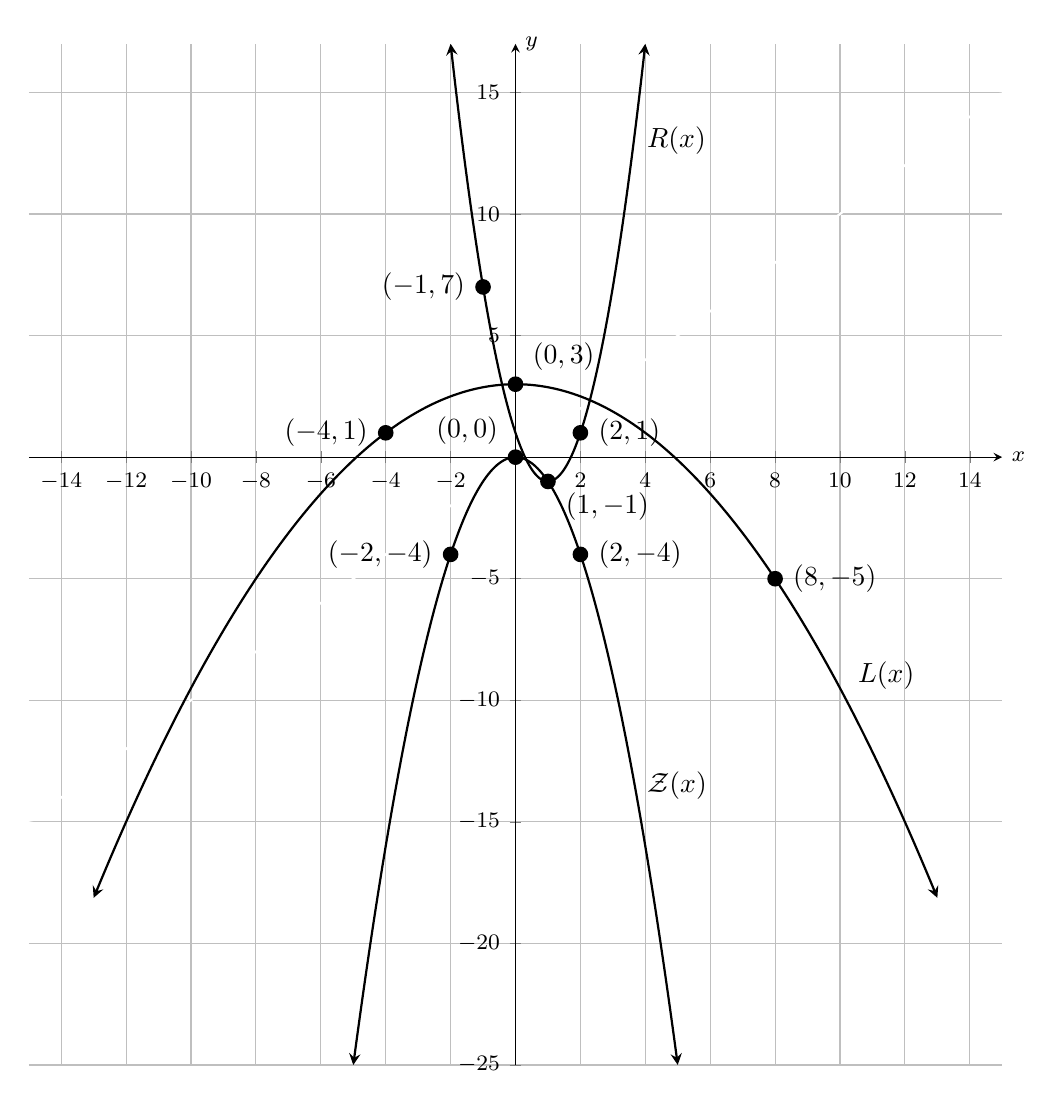
\begin{tikzpicture}
        \begin{axis}[
            my axis style,
            width=1.15\textwidth,
            height=1.2\textwidth,
            ylabel=$y$,
            grid
        ]

        \addplot[
            domain=-15:15,
            thick,
            white,
            <->
        ]
        {x};
        
        \addplot[
            domain=-5:5,
            thick,
            black,
            <->
        ]
        {-1*(-x)^2};

        \addplot[
            domain=-13:13,
            thick,
            black,
            <->
        ]
        {-2*(0.25*x)^2 + 3};

        \addplot[
            domain=-2:4,
            thick,
            black,
            <->
        ]
        {0.5*(-2*(x-1))^2 - 1};


        \fill[
            black
        ];

        \node[label={0:{\textcolor{black}{$(2,-4)$}}},circle,fill,inner sep=2pt] at (axis cs:2,-4) {};
        \node[label={180:{\textcolor{black}{$(-2,-4)$}}},circle,fill,inner sep=2pt] at (axis cs:-2,-4) {};
        \node[label={160:{\textcolor{black}{$(0,0)$}}},circle,fill,inner sep=2pt] at (axis cs:0,0) {};
        \node[label={0:{\textcolor{black}{$\mathcal{Z}(x)$}}},circle,inner sep=2pt] at (axis cs:3.5,-13.5) {};

        \node[label={180:{\textcolor{black}{$(-4,1)$}}},circle,fill,inner sep=2pt] at (axis cs:-4,1) {};
        \node[label={0:{\textcolor{black}{$(8,-5)$}}},circle,fill,inner sep=2pt] at (axis cs:8,-5) {};
        \node[label={25:{\textcolor{black}{$(0,3)$}}},circle,fill,inner sep=2pt] at (axis cs:0,3) {};
        \node[label={0:{\textcolor{black}{$L(x)$}}},circle,inner sep=2pt] at (axis cs:10,-9) {};

        \node[label={180:{\textcolor{black}{$(-1,7)$}}},circle,fill,inner sep=2pt] at (axis cs:-1,7) {};
        \node[label={350:{\textcolor{black}{$(1,-1)$}}},circle,fill,inner sep=2pt] at (axis cs:1,-1) {};
        \node[label={0:{\textcolor{black}{$(2,1)$}}},circle,fill,inner sep=2pt] at (axis cs:2,1) {};
        \node[label={0:{\textcolor{black}{$R(x)$}}},circle,inner sep=2pt] at (axis cs:3.5,13) {};

        \end{axis}
        \end{tikzpicture}
  \end{solution}
\end{qstn}

\newpage

\begin{qstn}
  \begin{solution}
    \textbf{Legend} : \textcolor{black}{$r(x) = -2f(x+1)$}, \,\,\textcolor{black}{$g(x)
    = -f(x-3)+1$}, \,\,\, \textcolor{black}{$R(x) = \frac{3}{2}f(-2x+4) - 2$}

        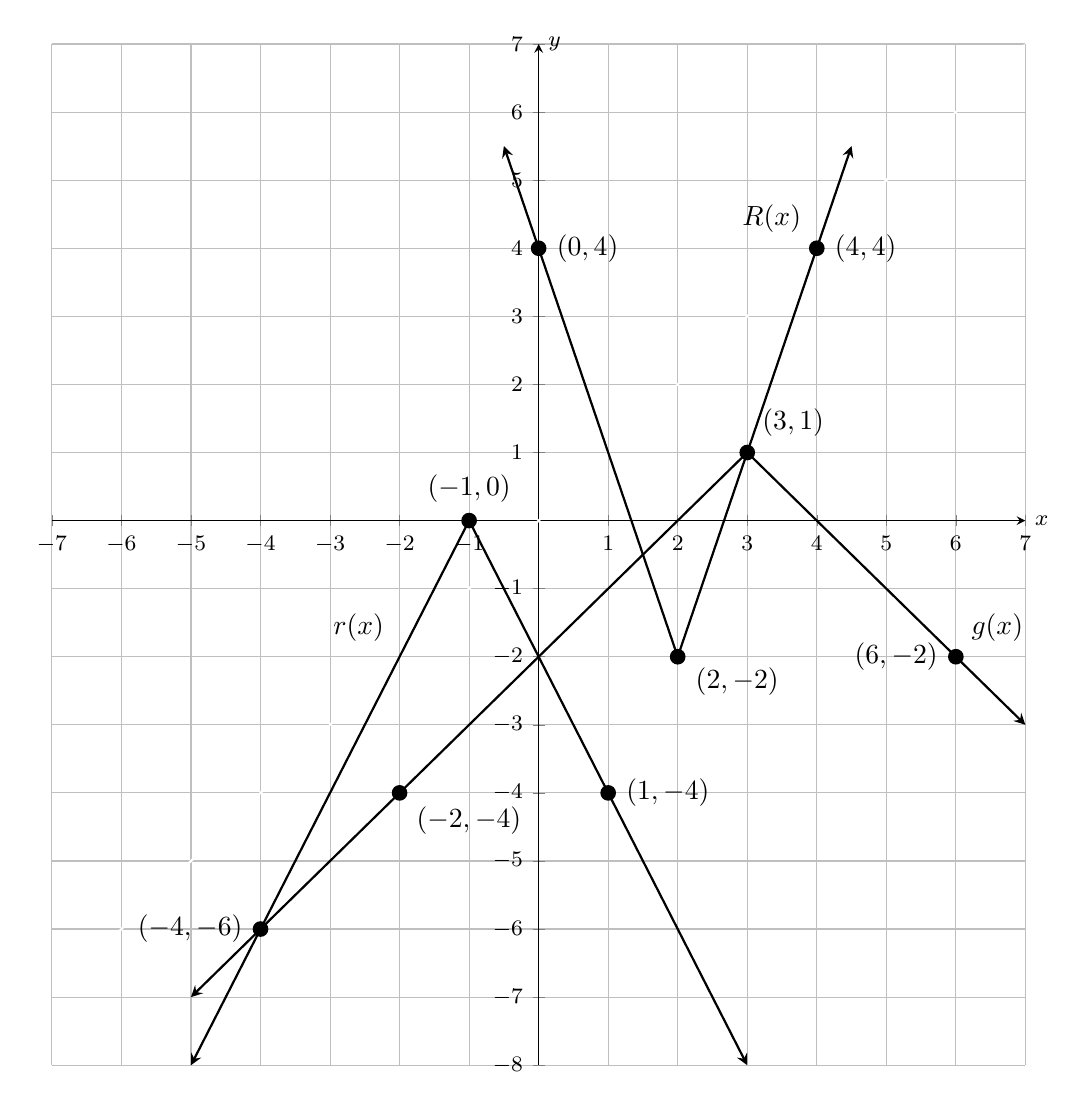
\begin{tikzpicture}
        \begin{axis}[
            my axis style,
            width=1.15\textwidth,
            height=1.2\textwidth,
            ylabel=$y$,
            grid
        ]

        \addplot[
            domain=-7:7,
            thick,
            white,
            <->
        ]
        {x};
        
        \addplot[
            domain=-5:7,
            thick,
            black,
            <->
        ]
        {-1*abs(x-3)+1};

        \addplot[
            domain=-5:3,
            thick,
            black,
            <->
        ]
        {-2*abs(x+1)};

        \addplot[
            domain=-0.5:4.5,
            thick,
            black,
            <->
        ]
        {1.5*abs(-2*x+4)-2};


        \fill[
            black
        ];

        \node[label={50:{\textcolor{black}{$(3,1)$}}},circle,fill,inner sep=2pt] at (axis cs:3,1) {};
        \node[label={-30:{\textcolor{black}{$(-2,-4)$}}},circle,fill,inner sep=2pt] at (axis cs:-2,-4) {};
        \node[label={180:{\textcolor{black}{$(6,-2)$}}},circle,fill,inner sep=2pt] at (axis cs:6,-2) {};
        \node[label={45:{\textcolor{black}{$g(x)$}}},circle,inner sep=2pt] at (axis cs:6,-2) {};

        \node[label={180:{\textcolor{black}{$(-4,-6)$}}},circle,fill,inner sep=2pt] at (axis cs:-4,-6) {};
        \node[label={90:{\textcolor{black}{$(-1,0)$}}},circle,fill,inner sep=2pt] at (axis cs:-1,0) {};
        \node[label={0:{\textcolor{black}{$(1,-4)$}}},circle,fill,inner sep=2pt] at (axis cs:1,-4) {};
        \node[label={135:{\textcolor{black}{$r(x)$}}},circle,inner sep=2pt] at (axis cs:-2,-2) {};

        \node[label={0:{\textcolor{black}{$(0,4)$}}},circle,fill,inner sep=2pt] at (axis cs:0,4) {};
        \node[label={350:{\textcolor{black}{$(2,-2)$}}},circle,fill,inner sep=2pt] at (axis cs:2,-2) {};
        \node[label={0:{\textcolor{black}{$(4,4)$}}},circle,fill,inner sep=2pt] at (axis cs:4,4) {};
        \node[label={135:{\textcolor{black}{$R(x)$}}},circle,inner sep=2pt] at (axis cs:4,4) {};

        \end{axis}
        \end{tikzpicture}
  \end{solution}
\end{qstn}

\newpage

\begin{qstn}
  \begin{solution}
    \textbf{Legend} : \textcolor{black}{$g(x) = -\frac{1}{2}f(4(x+4))+1$}.

        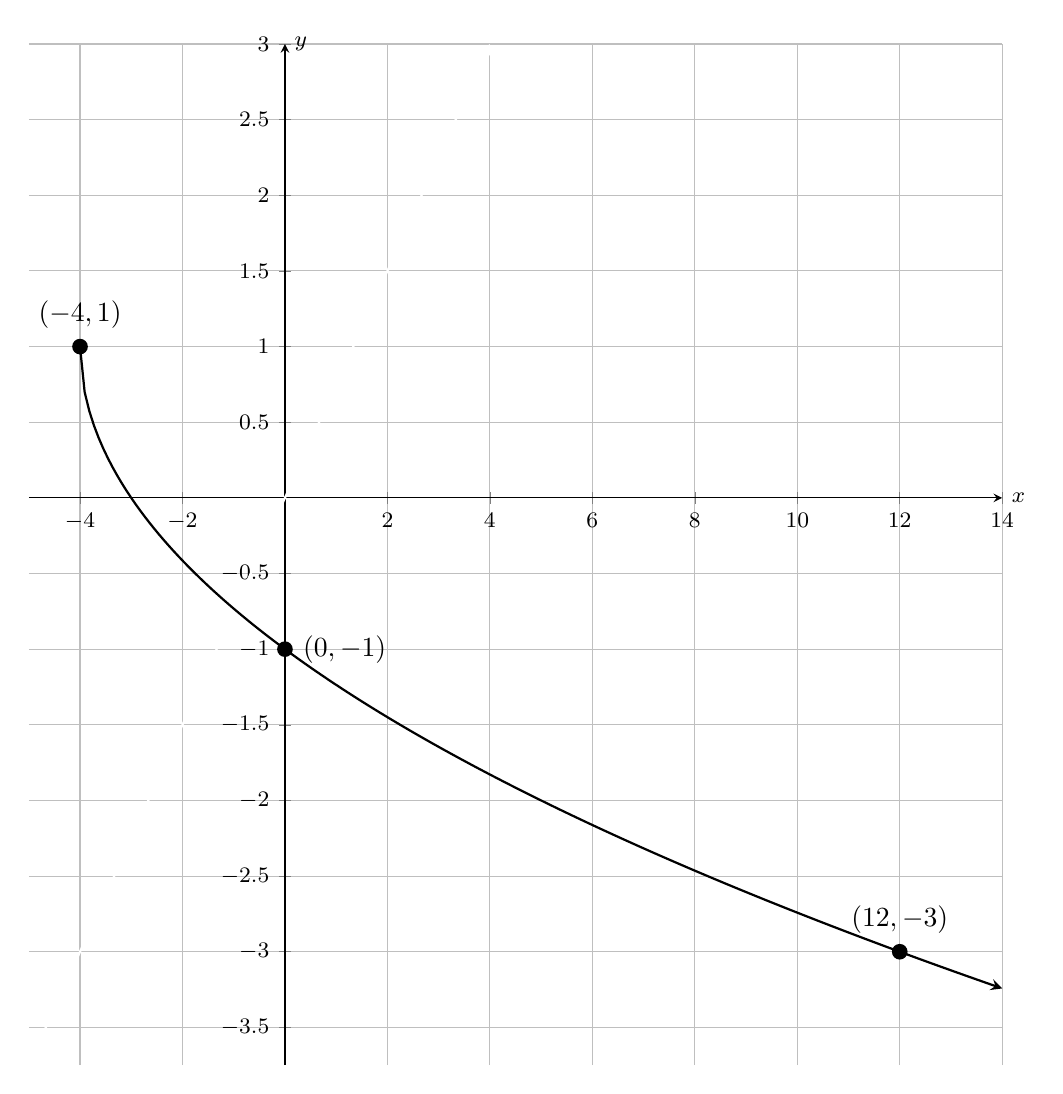
\begin{tikzpicture}
        \begin{axis}[
            my axis style,
            width=1.15\textwidth,
            height=1.2\textwidth,
            ylabel=$y$,
            grid
        ]

        \addplot[
            domain=-5:4,
            thick,
            white,
            <->
        ]
        {0.75*x};
        
        \addplot[
            domain=-4:14,
            thick,
            black,
            ->
        ]
        {-0.5*sqrt(4*x+16)+1};

        \fill[
            black
        ];

        \node[label={90:{\textcolor{black}{$(-4,1)$}}},circle,fill,inner sep=2pt] at (axis cs:-4,1) {};
        \node[label={0:{\textcolor{black}{$(0,-1)$}}},circle,fill,inner sep=2pt] at (axis cs:0,-1) {};
        \node[label={90:{\textcolor{black}{$(12,-3)$}}},circle,fill,inner sep=2pt] at (axis cs:12,-3) {};

        \end{axis}
        \end{tikzpicture}
  \end{solution}
\end{qstn}

\newpage

\begin{qstn}
  \begin{solution} \texttt{ }
  \begin{enumerate}[label=(\alph*)]
    \item $f(x) = -\frac{2}{3}(3x-6)^2-1 = -\frac{2}{3}\left( 3(x-2) \right) ^2 - 1$. The parent function here is
      $x^2$. The transformations,
      \begin{itemize}
        \item Reflection on the x-axis.
        \item Vertical compression by a factor of $\frac{3}{2}$.
        \item Horizontal compression by a factor of $3$.
        \item Horizontal shift, right $2$ units.
        \item Vertical shift, down $1$ unit.
      \end{itemize}

    \item $g(x) = 3\sqrt{-4x+12} + 9 =  3\sqrt{-4(x-3)} + 9$. The parent function here is
      $\sqrt{x} $.\\ The transformations are,
      \begin{itemize}
        \item Vertical stretch by a factor of $3$.
        \item Reflection on the y-axis.
        \item Horizontal compression by a factor of $4$.
        \item Horizontal shift, right $3$ units.
        \item Vertical shift, up $9$ units.
      \end{itemize}

    \item $h(x) = -4\left|\frac{1}{2}x + 1\right| = -4\left|\frac{1}{2}(x + 2)\right|$. The parent function here is
      $\left|x\right|$. The transformations are,
      \begin{itemize}
        \item Reflection on the x-axis.
        \item Vertical stretch by a factor of $4$.
        \item Horizontal stretch by a factor $2$.
        \item Horizontal shift, left $2$ units.
      \end{itemize}
  \end{enumerate}
    
  \end{solution}
\end{qstn}

\begin{qstn}
  \begin{solution} \texttt{   }
    \begin{enumerate}
      \item [(Q4.)]
    \begin{tasks}(4)
      \task II
      \task IV
      \task I
      \task III
    \end{tasks}

   \item [(Q61.)]
    \begin{tasks}(4)
      \task 3
      \task 1
      \task 2
      \task 4
    \end{tasks}

  \item [(Q61.)]
    \begin{tasks}(4)
      \task 2
      \task 3
      \task 1
      \task 4
    \end{tasks}
  \end{enumerate}

  \end{solution}
\end{qstn}


















\end{document}




























